
\documentclass{article}

% Language setting
% Replace `english' with e.g. `spanish' to change the document language
\usepackage[english]{babel}

% Set page size and margins
% Replace `letterpaper' with `a4paper' for UK/EU standard size
\usepackage[letterpaper,top=2cm,bottom=2cm,left=3cm,right=3cm,marginparwidth=1.75cm]{geometry}

% Useful packages
\usepackage{amsmath}
\usepackage{amssymb}
\usepackage{graphicx}
\usepackage[colorlinks=true, allcolors=blue]{hyperref}

\begin{document}


\section{The High-Luminosity LHC and Phase-2 of CMS}
% Tracker Phase-2: https://cds.cern.ch/record/2272264/files/CMS-TDR-014.pdf

\subsection{High-Luminosity LHC and CMS}
% cite https://cds.cern.ch/record/2714892/files/CMS-TDR-021.pdf
In order to sustain and extend the LHC's physics discovery program and maintain operability for a decade or more, the LHC is undergoing a major upgrade to the  High-Luminosity LHC (HL-LHC). In its final configuration, the HL-LHC will deliver a peak luminosity of $7.5 \times 10^{34}$ cm$^{-2}$ s$^{-1}$, potentially leading to total integrated luminosity of 4000 fb$^{-1}$ after ten years of operations, scheduled to begin in 2027 [CITE]. This integrated luminosity is about ten times the predicted luminosity reach of the LHC in its initial configuration. To maximize the discovery potential of this unprecedented amount of data, the CMS detector is undergoing Phase-2 upgrades in order to perform high-precision measurements and searches for physics beyond the Standard Model in the intense running conditions of the HL-LHC.

\subsection{The Phase-2 Level-1 Trigger}
% cite https://cds.cern.ch/record/2714892/files/CMS-TDR-021.pdf
To achieve the goals of the HL-LHC program and to ensure the collection of information-rich datasets in the HL-LHC, the Phase-2 upgrade of the CMS Level-1 Trigger must be upgraded in conjunction with the CMS sub-detectors and their readouts, to maintain physics selectivity. The HL-LHC will produce an intense hadronic environment corresponding to 200 simultaneous collisions per beam crossing, necessitating comprehensive upgrades of the trigger system outlined below.

% cite https://cds.cern.ch/record/2714892/files/CMS-TDR-021.pdf (page 7)
To profit from the extended coverage and increased granularity of the upgraded CMS detector, the latency of the L1 trigger system (time available to produce a L1 Accept signal) will be increased significantly from 3.8 $\mu$s to 12.5 $\mu$s, with an increased maximum output bandwidth of 750 kHz. [CITE]. With the increased latency, in addition to information from calorimeters and muon detectors (as in the Phase-1 system), information from the new tracker and high-granularity endcap calorimeter can also be included at L1 for the first time. This is illustrated in the functional diagram of the architecture of the Phase-2 trigger system in Fig. \ref{fig:phase-2-l1-architecture}. 

\begin{figure}[ht]
    \centering
    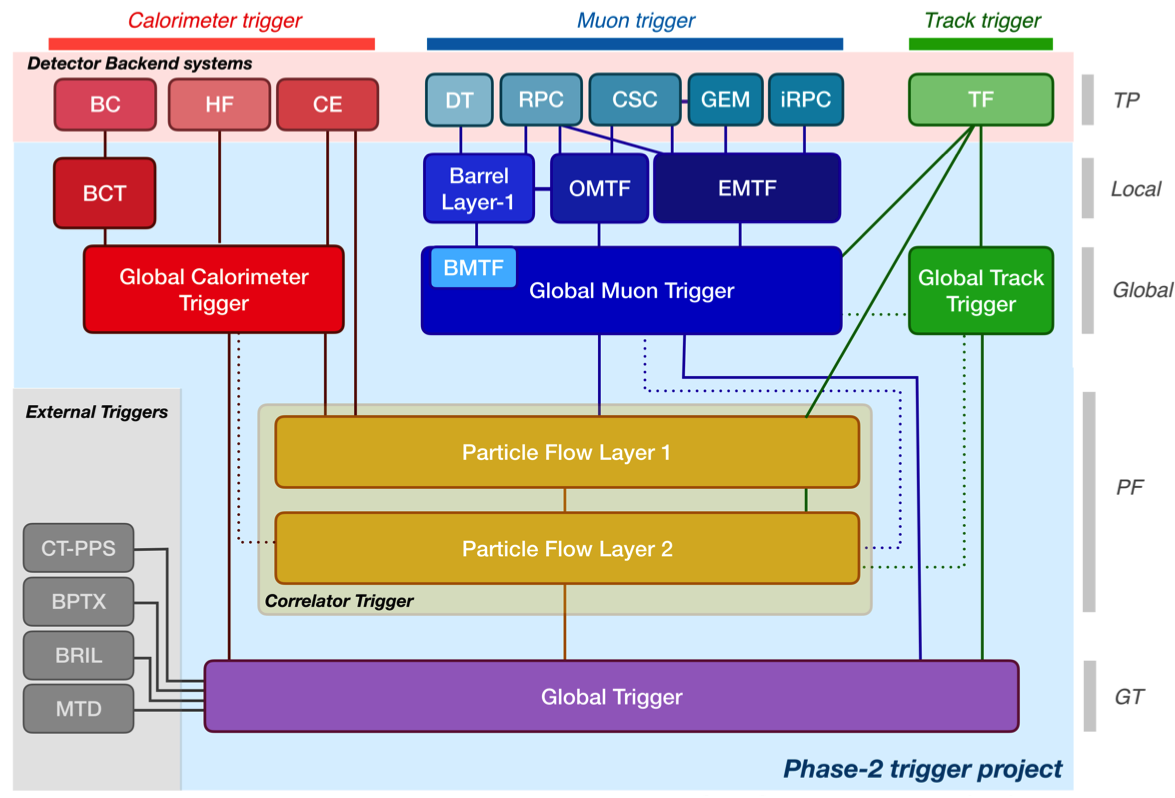
\includegraphics[width=15cm]{figures/phase-2-l1-architecture.png}
    \caption{Functional diagram of the CMS L1 Phase-2 upgraded trigger design from [CITE] https://cds.cern.ch/record/2714892/files/CMS-TDR-021.pdf, showing the four trigger paths: calorimeter, muon, track, and Particle Flow. For the first time, tracking information will be available as early as the L1 Trigger.}
    \label{fig:phase-2-l1-architecture}
\end{figure}

% cite https://cds.cern.ch/record/2714892/files/CMS-TDR-021.pdf (page 7)
The key feature of the Phase-2 L1 Trigger is the introduction of a correlator layer, where algorithms produce higher-level trigger objects by combining information from sub-detectors, with a selectivity approaching that of offline reconstruction in the HLT. Four independent data processing paths (grouped together in Fig. \ref{fig:phase-2-l1-architecture}) are implemented: tracking, calorimetry, muon systems, and particle-flow techniques:
\begin{itemize}
    \item \textbf{Calorimeter Trigger path:} (\textit{red}, Fig. \ref{fig:phase-2-l1-architecture}) A barrel calorimeter trigger (BCT) and the HGCAL backend are used to produce high-granularity information from the calorimeters to produce high-resolution clusters and identification variables used for later processing. Outputs from the BCT, HGCAL, and the HF are sent to a global calorimeter trigger (GCT), where caloriemter-only objects such as $e/\gamma$ candidates, hadronically decaying tau lepton candidates, jets, and energy sums are built.
    \item \textbf{Track Trigger path:} (\textit{green}, Fig. \ref{fig:phase-2-l1-architecture}) Tracks from the Outer Tracker are reconstructed in the track finder (TF) processors as part of the detector backend. A global track trigger (GTT) will reconstruct the primary vertices of the event, along with tracker-only based objects, such as jets and missing transverse momentum.
    \item \textbf{Muon Trigger path:} (\textit{blue}, Fig. \ref{fig:phase-2-l1-architecture}) Trigger primitives are processed by muon track finder algorithms, again separated into the barrel (barrel muon track finder, BMTF), overlap (overlap muon track finder, OMTF), and endcap (endcap muon track finder, EMTF). Standalone muons and stubs containing information such as position, bend angle, and timing, as well as L1 tracks, are sent to the global muon trigger (GMT).
    \item \textbf{Particle-Flow Trigger path:} (\textit{yellow}, Fig. \ref{fig:phase-2-l1-architecture}) The correlator trigger (CT) aims to approach the performance of offline Particle Flow, and is implemented in two layers. ``Layer-1'' produces the particle-flow candidates from matching calorimeter clusters and tracks. ``Layer 2'' builds and sorts final trigger objects and applies additional identification and isolation criteria.
\end{itemize}

% cite for MTD https://cds.cern.ch/record/2296612/files/LHCC-P-009.pdf
The outputs from the above trigger paths are combined in the Global Trigger (GT) (\textit{purple}, Fig. \ref{fig:phase-2-l1-architecture}), which calculates the final trigger decision (Level-1 Accept), transmitting it to the Trigger Control and Distribution System (TCDS), which distributes it to the detector backend systems, initiating the readout to the DAQ. The GT also provides the interface to external triggers (\textit{grey}, Fig. \ref{fig:phase-2-l1-architecture}), such as triggers for the precision proton spectrometer (PPS), beam position and timing monitors (BPTX), and luminosity and beam monitoring (BRIL) detectors. The design of the Phase-2 Level-1 Trigger allows for future inclusion of triggering information, for instance information about minimum ionizing particles (MIPs) from the MIP Timing Detector (MTD).



\end{document}